\documentclass{beamer}
\mode<presentation>

\usetheme{Marburg}
\setbeamertemplate{navigation symbols}{}
\setbeamercovered{transparent}

\usepackage[italian]{babel}
\usepackage[utf8]{inputenc}
\usepackage{graphics}
\usepackage{textcomp}
\usepackage{epstopdf}
\usepackage{times}
\usepackage{multirow}
\usepackage{threeparttable}
\usepackage{multimedia}
\usepackage{array}
\usepackage{tikz}
\usepackage{csquotes}
\usepackage{amsmath,amsthm, amssymb, latexsym}
\usepackage[absolute,overlay]{textpos}

\urlstyle{same}
\usetikzlibrary{decorations.pathmorphing}
\usetikzlibrary{shapes,arrows}
%\usepackage{lmodern}  
\usepackage[T1]{fontenc}
\usepackage[utf8]{inputenc}
\usepackage{booktabs}
\usepackage{array}
\usepackage{epstopdf}
\usepackage{multirow}
\usepackage{tabularx}
\usepackage{ragged2e}
\usepackage{everysel}

%\usepackage[symbol]{footmisc}
\renewcommand{\thefootnote}{\fnsymbol{footnote}}

\usepackage{caption}
\usepackage{hyperref}

\usefonttheme{structurebold}
\usefonttheme[onlymath]{serif}

\setbeamertemplate{bibliography item}{\insertbiblabel}
\setbeamercolor{bibliography item}{fg=black}
\setbeamercolor*{bibliography entry title}{fg=black}

\newcommand{\ac}{\\ \vspace{0.2cm}}
\newcommand{\de}{\,\textrm{d}}

\title[Commissioning TPS]{Commissioning di un sistema di elaborazione di piani di trattamento radioterapici\\\vspace*{.05cm}
        per tecniche 3D-CRT, IMRT,\\\vspace*{.1cm} VMAT e Radioterapia Adattiva}
\institute{\tiny Università dell'Aquila\ac Tesi di Specializzazione\\ Scuola di Specializzazione in Fisica Medica}
\date{05.Lug.2016}
\author{\textit{Alessandro Savini}}




\makeatletter
\setbeamertemplate{sidebar \beamer@sidebarside}
{
\beamer@tempdim=\beamer@sidebarwidth%
\advance\beamer@tempdim by -6pt%
{\usebeamerfont{title in sidebar}%
  \vskip1.5em%
  \hskip3pt%
  \usebeamercolor[fg]{title in sidebar}%
  \insertshorttitle[width=\beamer@tempdim,center,respectlinebreaks]\par%
  \vskip1.25em%
}%
{%
  \hskip3pt%
  \usebeamercolor[fg]{author in sidebar}%
  \usebeamerfont{author in sidebar}%
  \insertshortauthor[width=\beamer@tempdim,center,respectlinebreaks]\par%
  \vskip1.25em%
}%
\insertverticalnavigation{\beamer@sidebarwidth}%
\vfill
\ifx\beamer@sidebarside\beamer@lefttext%
\else%
  \usebeamercolor{normal text}%
  \llap{\usebeamertemplate***{navigation symbols}\hskip0.1cm}%
  \vskip2pt%
\fi%
%\hskip8pt

\includegraphics[width=2cm,keepaspectratio]{./img/logo-univaq.png}\\

\includegraphics[width=2cm,keepaspectratio]{./img/logoASL1.png}~%
}
\makeatother


\usepackage[style=numeric-comp, backend=biber, citestyle=numeric-comp, maxcitenames=1, mincitenames=1, doi=false,isbn=false,url=false,sorting=none]{biblatex}

\addbibresource{../bibliografia/Th.bib}
\addbibresource{../bibliografia/Th-adapt.bib}
\renewcommand*{\bibfont}{\tiny}

\definecolor{Dgreen}{HTML}{007800}

\setbeamercolor{block body}{bg=red!30,fg=black}


\newcommand*{\boxcolor}{red}
\makeatletter
\renewcommand{\boxed}[1]{\textcolor{\boxcolor}{%
\tikz[baseline={([yshift=-1ex]current bounding box.center)}] \node [rectangle, minimum width=1ex,rounded corners,draw] {\normalcolor\m@th$\displaystyle#1$};}}

\newcommand{\srcsize}{\@setfontsize{\srcsize}{5pt}{5pt}}
\makeatother



\begin{document}

\begin{frame}

\includegraphics[width=2cm,keepaspectratio]{./img/logo-univaq.png} \hfill

\includegraphics[width=1cm,keepaspectratio]{./img/logo_dept.jpg} \hfill

\includegraphics[width=2cm,keepaspectratio]{./img/logoASL1.png}
\titlepage
\end{frame}



\section[Intro RT fasci esterni]{Introduzione alla radioterapia a fasci esterni}

\begin{frame}{Introduzione RT a fasci esterni}
\begin{center}
\structure{Acceleratore lineare (LINAC)}\\ \vspace{.2cm}
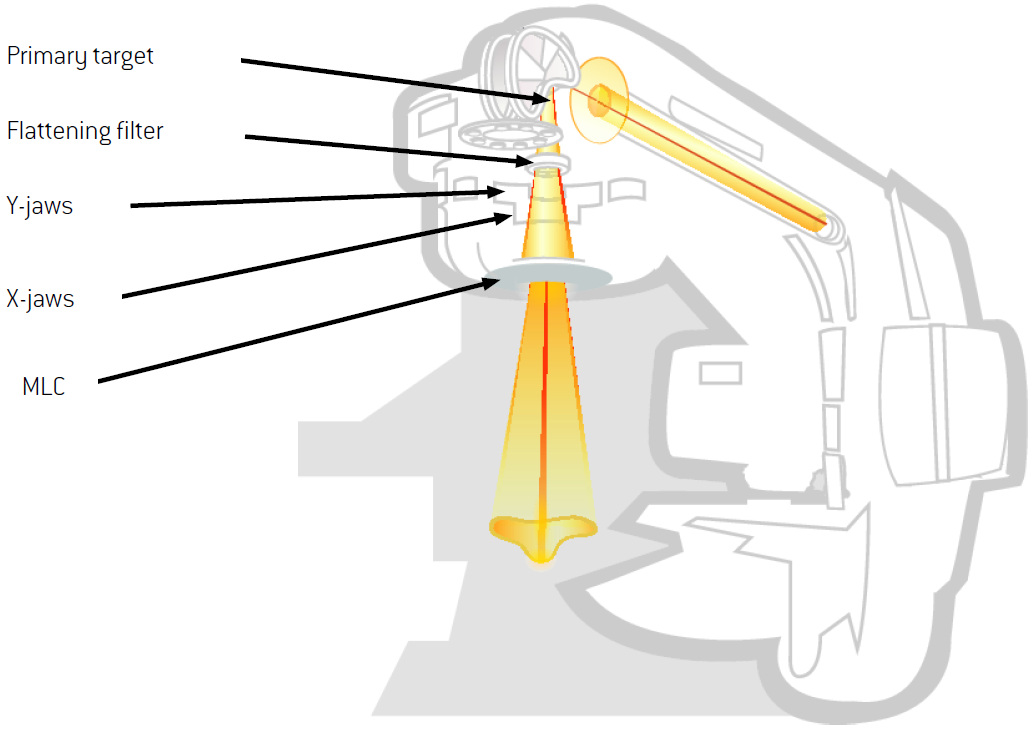
\includegraphics[width=.6\textwidth]{../cap1/linac.PNG}
\end{center}
\footnotesize
\structure{Radioterapia a fasci esterni:} tecnica medica che fa impiego di radiazioni ionizzanti per il trattamento di patologie (neoplasie maligne principalmente).\ac 
\structure{Dose fisica:} al pari della dose farmacologica è la quantità utilizzata per ottenere l'effetto terapeutico.
$$D = \frac{\de \bar{\varepsilon}}{\de m} \qquad\qquad \text{Unità: J\,kg}^{-1} \equiv \text{Gray [Gy]}$$
\end{frame}

\begin{frame}{Introduzione RT a fasci esterni}
\begin{center}
\small
\structure{Principali interazioni radiazione-paziente}\\ \vspace{.2cm}
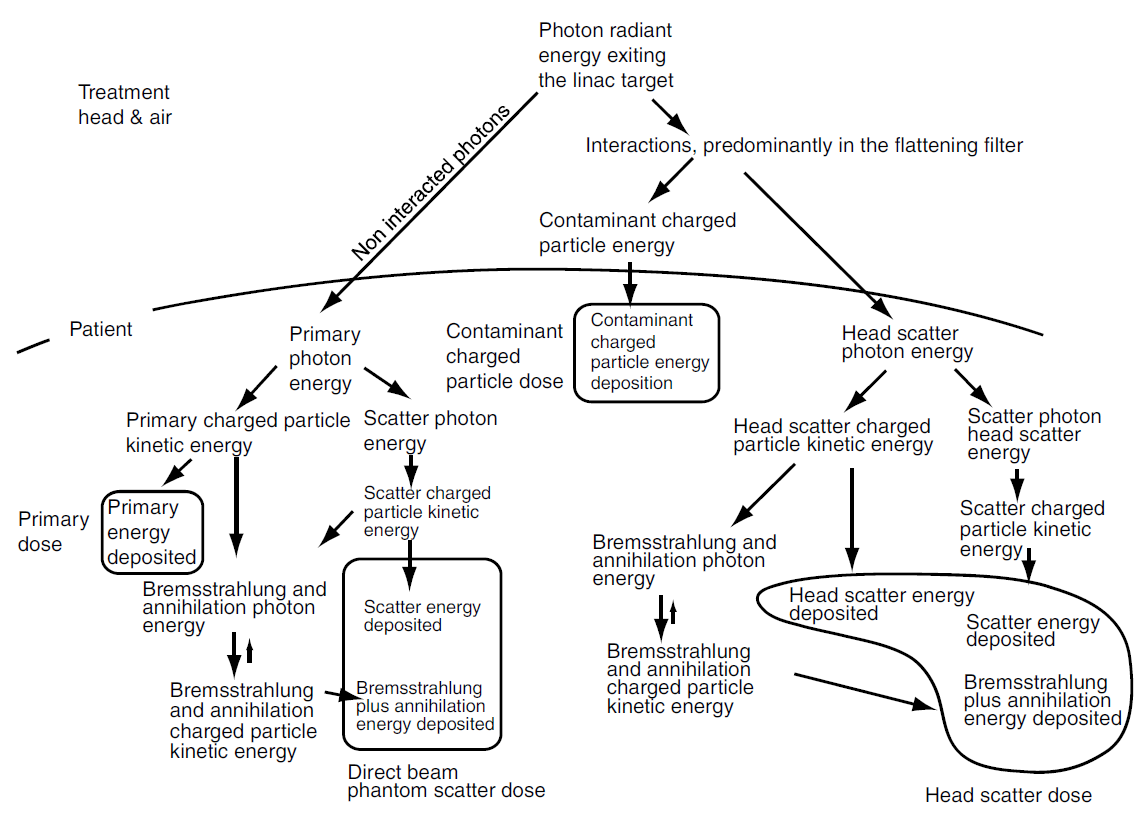
\includegraphics[width=.8\textwidth]{../cap1/processes.PNG}
\end{center}
\end{frame}



\begin{frame}{Introduzione RT a fasci esterni}
\begin{center}
\small
%\structure{Principali interazioni radiazione-paziente}\\ \vspace{.2cm}
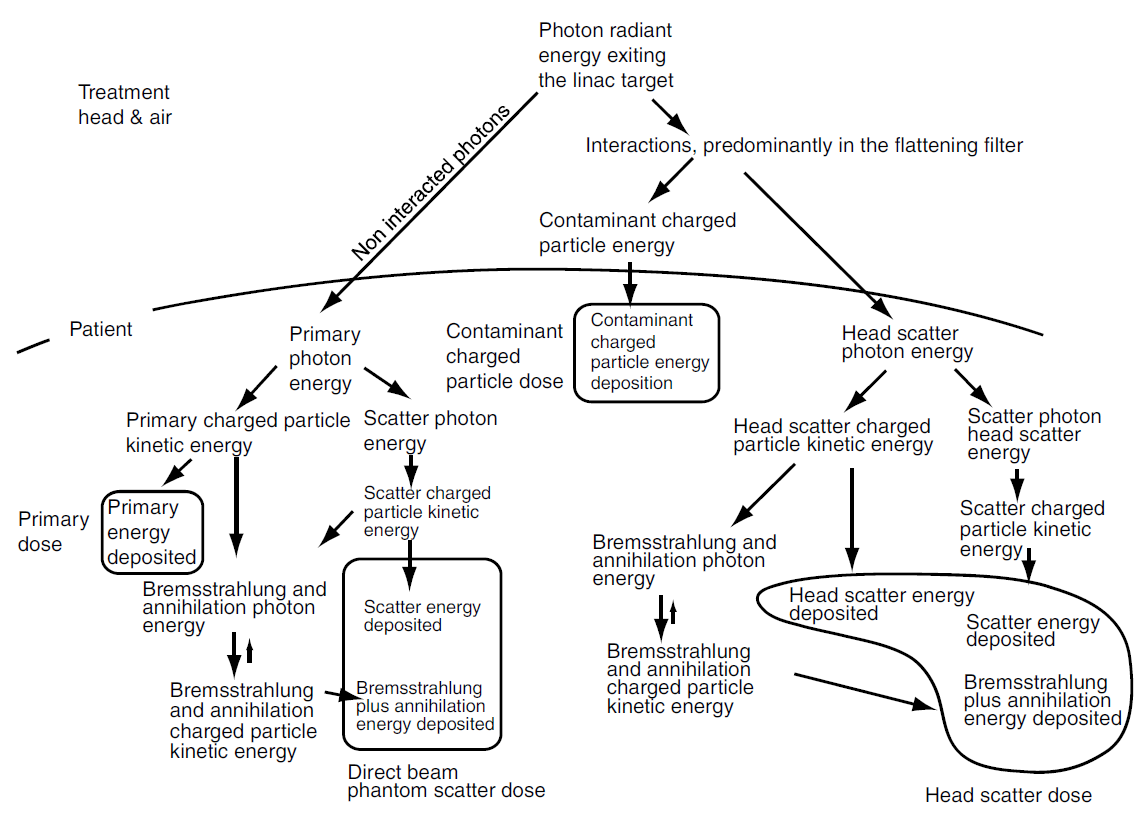
\includegraphics[width=.6\textwidth]{../cap1/processes.PNG}
\end{center}
\begin{itemize}
\scriptsize
\item \alert{Dose primaria:} originata dalla parte di fascio che non ha interagito nella testata $\Rightarrow$ $\sim 70\%$ della dose totale).
\item \alert{\textit{Head scatter dose}:} originata dalla parte di fascio che ha interagito nella testata (\textit{flattening filter}) $\Rightarrow$ $\sim 5\div 10\%$ della dose totale.
\item \alert{\textit{Phantom scatter dose}:} dovuta ai processi di scatter all'interno del paziente dalla parte di fascio che ha interagito nella testata (\textit{flattening filter}) $\Rightarrow$ $\sim 30\%$ della dose totale.
\item \alert{Dose da contaminazione:} originata dalla parte di fascio non fotonica (prevalentemente elettroni) $\Rightarrow$ comparabile con la dose primaria solo nei primi $mm$ di tessuto.
\end{itemize}
\end{frame}

\section{Algoritmi di calcolo della dose}

\begin{frame}{Algoritmi di calcolo della dose}
\begin{columns}
\column{.48\textwidth}
\centering
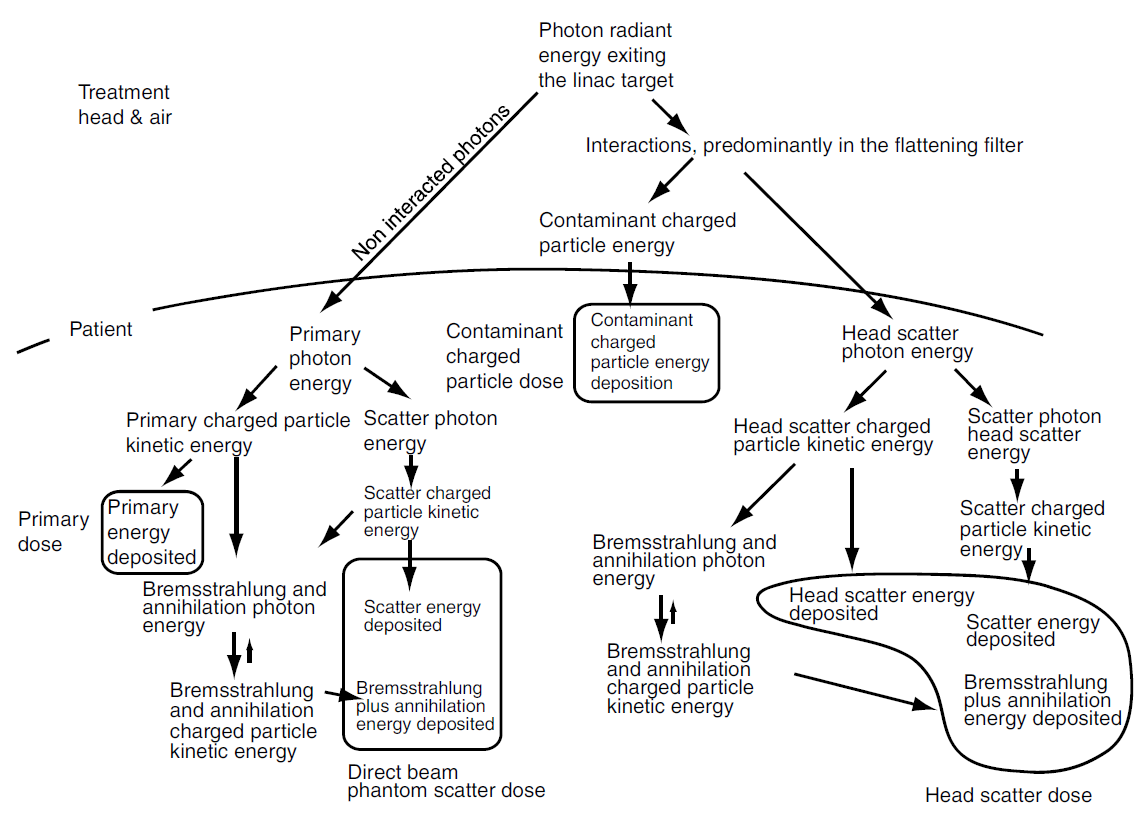
\includegraphics[width=\textwidth]{../cap1/processes.PNG}
\column{.05\textwidth}
\large$$\Rightarrow$$
\column{.48\textwidth}
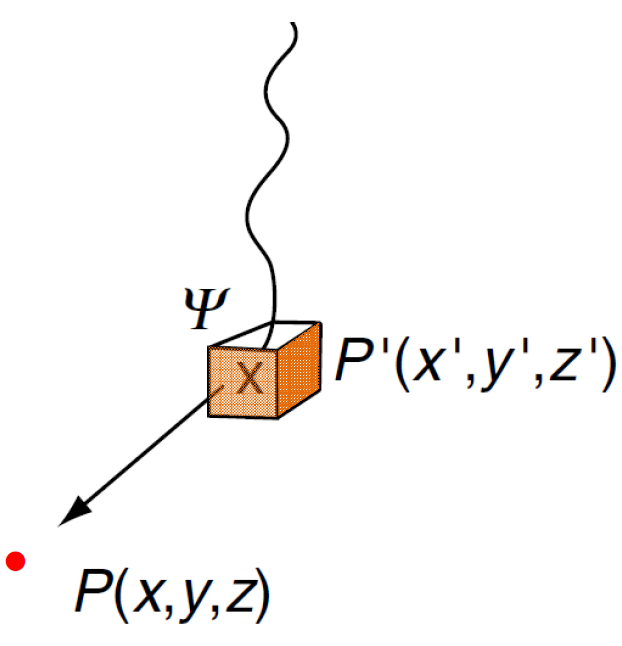
\includegraphics[width=.5\textwidth]{../cap1/superp1.png}
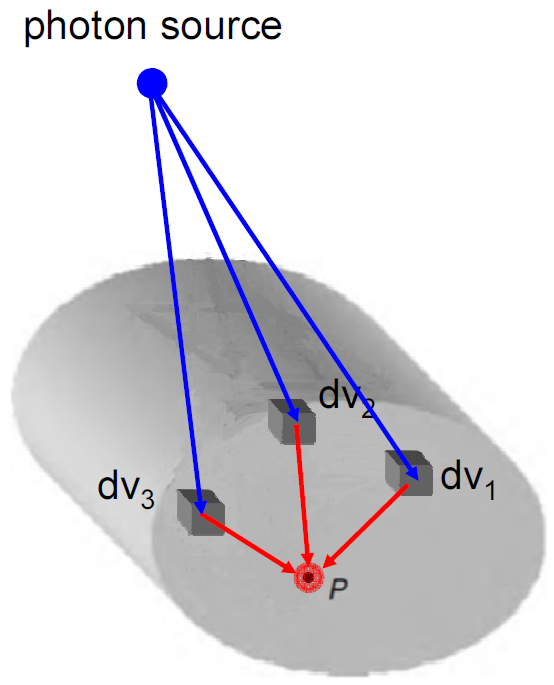
\includegraphics[width=.5\textwidth]{../cap1/superp2.png}
\end{columns}
\vspace{.5cm}
\small $$D(x,y,z) = \int_V T(P')\,s(P'\rightarrow P)\, \de V'$$
\begin{itemize}
\scriptsize
\item \structure{$D(x,y,z):$} dose nel punto $P$.
\item \structure{$T(P'):$} \textit{Total-Energy-Released-in-Matter} (TERMA) $\rightarrow$ fluenza di energia ($\Psi\, [J\, m^{-2}]$) $\times$ coefficiente assorbimento massico ($\mu/\rho\,[kg^{-1}\, m^{2}]$) nel punto $P'$ .
\item \structure{$s(P'\rightarrow P):$} \textit{funzione di scatter} $\rightarrow$ quantità di energia assorbita in $P$ dovuta ad un'interazione di un fotone con energia fissata nel punto $P'$.
\end{itemize}
\end{frame}


\begin{frame}{Algoritmi di calcolo della dose}
\small $$D(x,y,z) = \int_V T(P')\,s(P'\rightarrow P)\, \de V'$$\\ \vspace{.5cm}
\structure{Step per il calcolo della dose:}
\begin{itemize}
\footnotesize
\item Calcolo della fluenza di energia.
\item Calcolo della distribuzione di TERMA.
\item Applicazione delle funzioni di scatter.
\item Somma del contributo dovuto alle particelle di contaminazione (elettroni).
\end{itemize}

\end{frame}


\begin{frame}{Algoritmi di calcolo della dose}
\scriptsize
\begin{itemize}
\setbeamercolor{item}{fg=red}
\scriptsize
\item \color{red}Calcolo della fluenza di energia e del TERMA.
\end{itemize}
\vspace{.2cm}
\scriptsize
\begin{enumerate}
\item[1.] Proiezione delle sorgenti attraverso i collimatori sul \textit{fluence-plane}.
\end{enumerate}
\begin{columns}
\column{.4\textwidth}
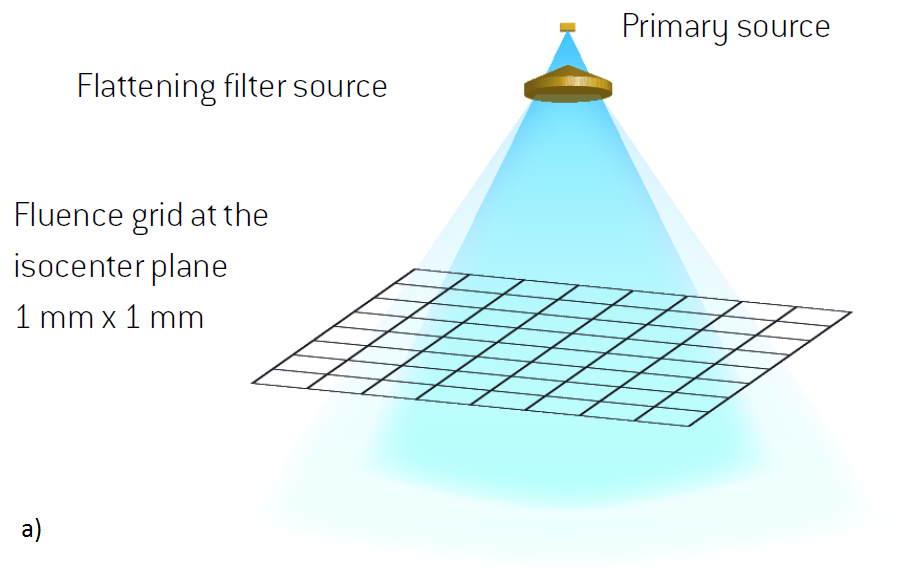
\includegraphics[width=\textwidth]{../cap1/twosources.png}
\column{.3\textwidth}
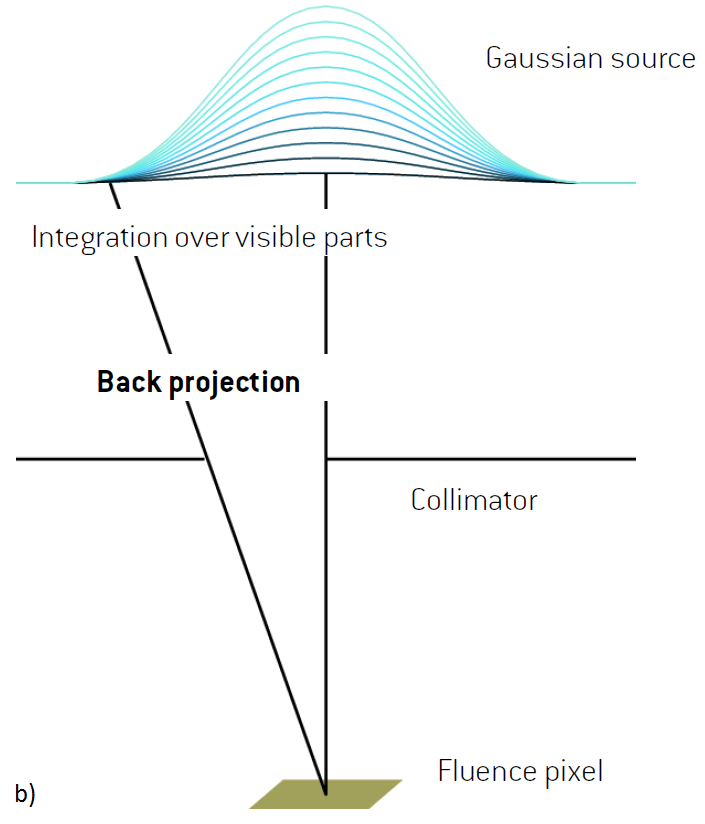
\includegraphics[width=\textwidth]{../cap1/source_int.png}
\column{.3\textwidth}
\includegraphics[width=\textwidth]{../cap1/TERMA_isoPatient.eps}
\end{columns}

\uncover<2->{
\scriptsize
\begin{enumerate}
\item[2.] CT del paziente $\rightarrow$ mappa del coefficiente di attenuazione ($\mu/\rho$) proiezione ed attenuazione della fluenza all'interno del paziente $\rightarrow$ distribuzione di TERMA.
\end{enumerate}
\vspace{-.3cm}

\begin{align*}
TERMA(\vec{r'},E) &= \frac{\mu}{\rho}(\vec{r'},E) \cdot \Psi(\vec{r'},E)\\
				  &= \frac{\mu}{\rho}(\vec{r'},E) \cdot \frac{|\vec{r_0}|^2}{|\vec{r'}|^2}\Psi(\vec{r_0},E)\,\exp{\left( -\int_{\vec{r_0}}^{\vec{r'}} \mu(\vec{r'},E) \de l \right)}
\end{align*}
}
\end{frame}



\begin{frame}{Algoritmi di calcolo della dose}
\small $$D(x,y,z) = \int_V T(P')\,s(P'\rightarrow P)\, \de V'$$\\ \vspace{.5cm}
\structure{Step per il calcolo della dose:}
\begin{itemize}
\footnotesize
\item Calcolo della fluenza di energia.
\item Calcolo della distribuzione di TERMA.
\setbeamercolor{item}{fg=red}
\item \alert{Applicazione delle funzioni di scatter.}
\setbeamercolor{item}{fg=structure}
\item Somma del contributo dovuto alle particelle di contaminazione (elettroni).
\end{itemize}
\end{frame}




\begin{frame}{Algoritmi di calcolo della dose}
\scriptsize
\begin{itemize}
\setbeamercolor{item}{fg=red}
\scriptsize
\item \color{red}Applicazione delle funzioni di scatter.
\end{itemize}
\vspace{.2cm}
\scriptsize
\begin{enumerate}
\item[1.] Calcolo \textit{Monte Carlo} della funzione di scatter generata forzando l'interazione di un fotone ad energia fissata in un punto di un mezzo omogeneo $\sim{}\infty$ esteso (ove si verifica la condizione di equilibrio di particelle cariche o CPE).
\end{enumerate}
\begin{columns}
\column{.4\textwidth}
\centering
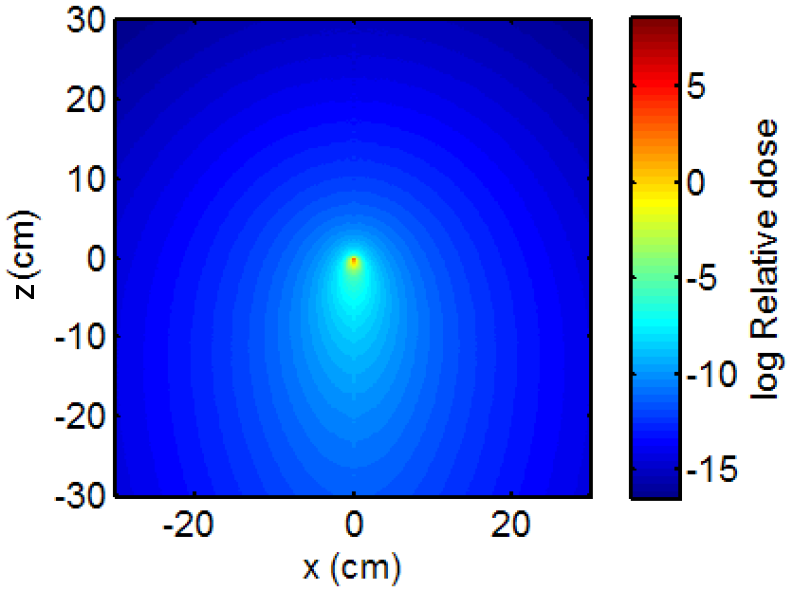
\includegraphics[width=\textwidth]{../cap1/kern_ray1.png}
\column{.4\textwidth}
\centering
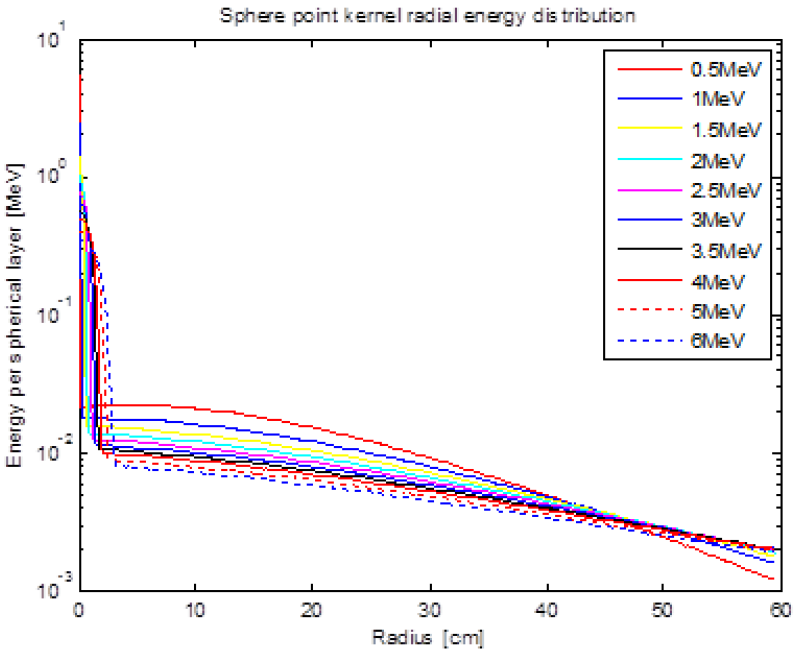
\includegraphics[width=\textwidth]{../cap1/kern_ray2.png}
\end{columns}

\uncover<2->{
\scriptsize
\begin{enumerate}
\item[2.] Risoluzione dell'integrale per il calcolo della dose totale.
\end{enumerate}
$$D(x,y,z) = \int_V T(P')\,s(P'\rightarrow P)\, \de V'\, \overset{\scriptscriptstyle CPE}{=}\, \underbrace{\int_V T(P')\,s(P' - P)\, \de V'}_{Int.Convoluzione}$$
}
\end{frame}


\begin{frame}{Algoritmi di calcolo della dose}

\small \begin{equation}
D(x,y,z) = \int_V T(P')\,s(P'\rightarrow P)\, \de V'
\label{eq:conv}
\end{equation}

\vspace{.5cm}
\structure{Metodi di risoluzione (computazionali):}
\begin{itemize}
\small
\item Somma diretta $\rightarrow$ $\sim N^6$ operazioni.
\begin{itemize}
\scriptsize
\item $N:$ numero di voxel della griglia di dose.
\item Estensione al caso disomogeneo $\rightarrow$ ulteriori $N$ operazioni.
\end{itemize}
\item Teorema di convoluzione $\rightarrow$ $\sim N^3\log_2 N$ operazioni.
\begin{itemize}
\scriptsize
\item Applicabile senza correzioni solo al caso omogeneo per il quale vale che $s(P'\rightarrow P) = s(P'- P)$ $\rightarrow$ (invariante spaziale, condizioni CPE).
\end{itemize}
\item \textit{Collapsed-cone-convolution} $\rightarrow$ $\sim MN^2$ operazioni.
\begin{itemize}
 \scriptsize 
\item $M:$ numero di direzioni di discretizzazione angolare.
\item Approssimabile per trattare il caso disomogeneo (assenza di CPE) con ulteriori $N$ operazioni.
\end{itemize}
\end{itemize}
\end{frame}


\begin{frame}{Algoritmi di calcolo della dose}
\small
\centering
\alert{\textit{Collapsed-cone-convolution}}\\\vspace{.3cm}
\begin{columns}[t]
\column{.5\textwidth}
\centering
\includegraphics[height=4cm]{../cap1/Kernel_RayTr.eps}\\\vspace{.5cm}
\scriptsize
\structure{Discretizzazione angolare sempice}
\begin{itemize}
\scriptsize
\item Necessario un alto numero di direzioni per limitare l'errore di \textit{under-sampling}.
\end{itemize}

\column{.5\textwidth}
\centering
\includegraphics[height=4cm]{../cap1/Kernel_CCC.eps}\\\vspace{.5cm}
\scriptsize
\structure{Discretizzazione \textit{collapsed-cone}}
\begin{itemize}
\scriptsize
\item Contributo di un settore conico collassato lungo l'asse.
\item Necessario un campionamento angolare ridotto.
\end{itemize}
\end{columns}
\end{frame}



\begin{frame}[t]{Algoritmi di calcolo della dose}
\small
{\centering
\alert{\textit{Collapsed-cone-convolution}\\
\footnotesize Generalizzazione al caso poli-energetico e disomogeneo} \\ \vspace{.5cm}
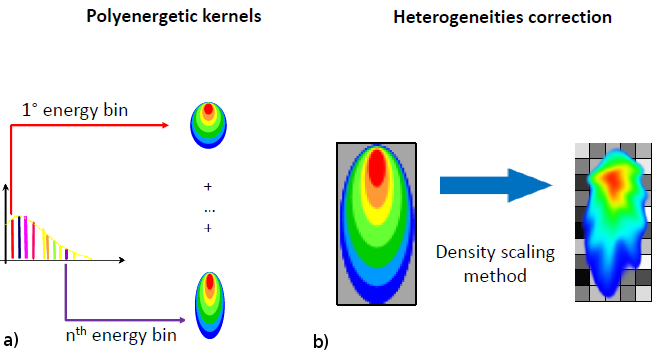
\includegraphics[width=.7\textwidth]{../cap1/kern_trans.png}\\
\scriptsize
\begin{itemize}
\item[a)] \structure{\normalfont{Funzione di scatter polienergetica}} $\rightarrow$ media di kernel polienergetici pesati con lo spettro di energia del fascio primario.
\item[b)] \structure{\normalfont{Density-scaling:}} $\rightarrow$ forma dei kernel scalata con la lunghezza radiologica ($Lunghezze\,\rightarrow\,Lunghezze \times Densit\grave{a}$)
\end{itemize}
}
\only<2->{\color{Dgreen} \scriptsize \bf Tutto ciò per evitare di ricalcolare le funzioni di scatter con metodo MC per ogni possibile situazione!}
\end{frame}



\begin{frame}{Algoritmi di calcolo della dose}
\begin{columns}[t]
\column{.49\textwidth}
%\begin{center}
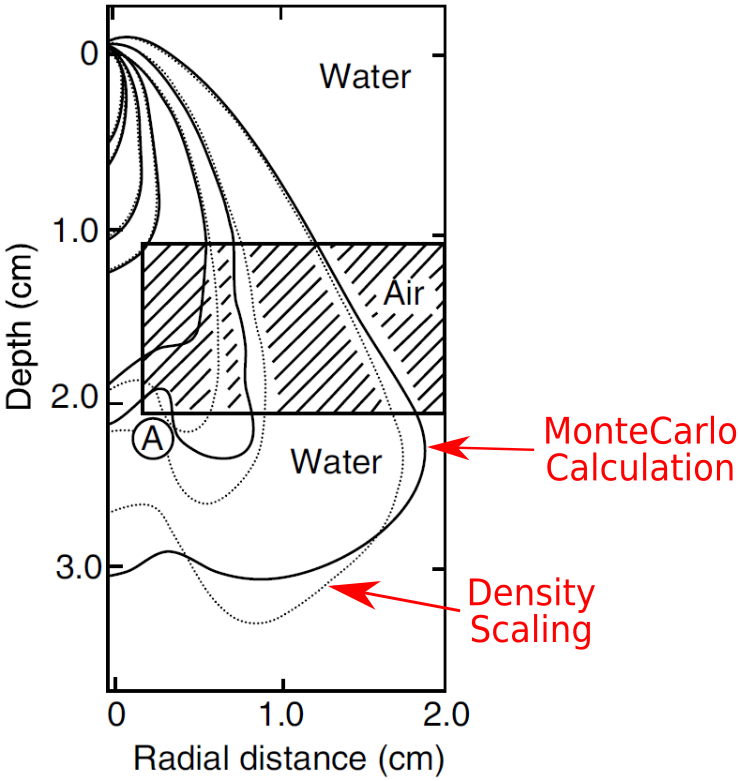
\includegraphics[width=\textwidth]{../cap1/kern_dens_pres.png}
%\end{center}
\scriptsize
\begin{itemize}
\item Metodo del \textit{density-scaling} $\rightarrow$ discrepanze fino al 50\% sul singolo kernel rispetto al MC (punto A).
\end{itemize}
\column{.03\textwidth}
%\vspace{-3cm}
%\large $$\Rightarrow$$
\column{.5\textwidth}
%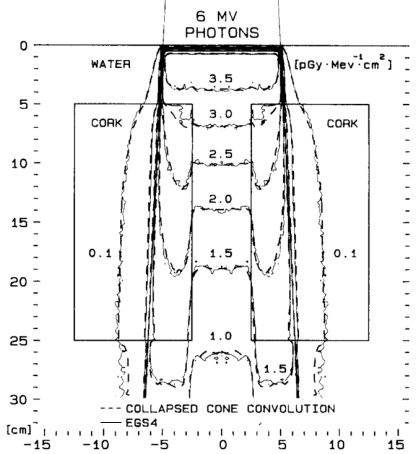
\includegraphics[width=\textwidth]{../cap1/kern_dens2_pres.png}
%\scriptsize
%\begin{itemize}
%\item Tuttavia su un grande numero di interazioni $\rightarrow$ effetto di \textit{averaging}.
%\item Discrepanze rispetto al MC significative (\sim 10\%) solo alle interfacce.
%\end{itemize}
\end{columns}
\end{frame}


\begin{frame}{Algoritmi di calcolo della dose}
\begin{columns}[t]
\column{.49\textwidth}
%\begin{center}
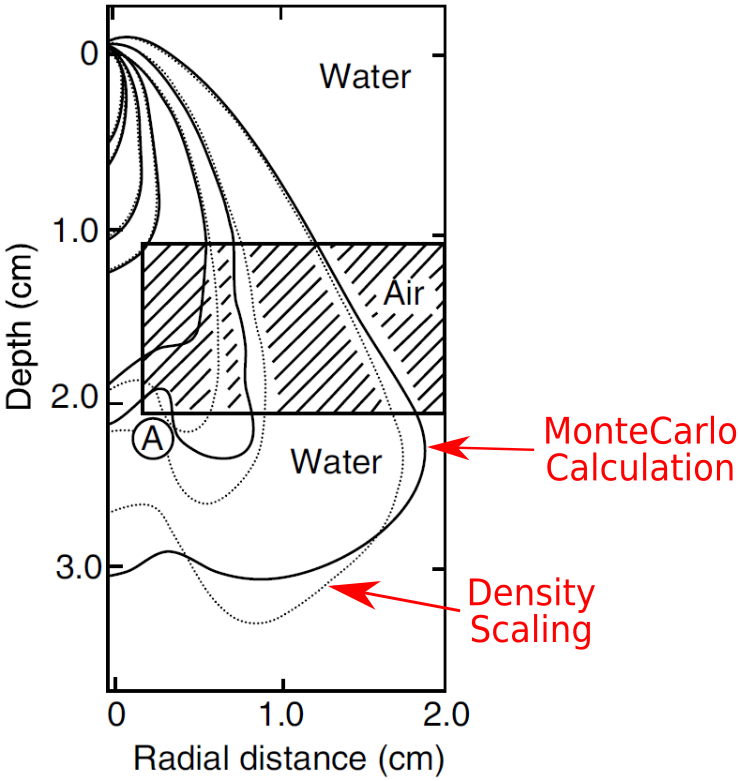
\includegraphics[width=\textwidth]{../cap1/kern_dens_pres.png}
%\end{center}
\scriptsize
\begin{itemize}
\item Metodo del \textit{density-scaling} $\rightarrow$ discrepanze fino al 50\% sul singolo kernel rispetto al MC (punto A).
\end{itemize}
\column{.03\textwidth}
\vspace{-3cm}
\large $$\Rightarrow$$
\column{.5\textwidth}
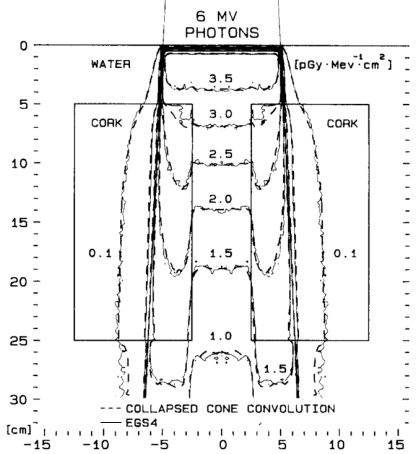
\includegraphics[width=\textwidth]{../cap1/kern_dens2_pres.png}
\scriptsize
\begin{itemize}
\item Tuttavia su un grande numero di interazioni $\rightarrow$ effetto di \textit{averaging}.
\item Discrepanze rispetto al MC significative ($\sim 10\%$) solo alle interfacce (assenza di CPE).
\end{itemize}
\end{columns}
\end{frame}



\section[Modellizzazione del LINAC]{Modellizzazione fisica del LINAC nel TPS RayStation}
\begin{frame}{Indice}
\tableofcontents[currentsection]
\end{frame}

\begin{frame}{Modellizzazione del LINAC}
\small
\structure{Step da seguire:}
\begin{itemize}
\item Acquisizione di misure dosimetriche del fascio di radiazione prodotto dal LINAC.
\item \textit{Tuning} dei parametri del modello fisico del LINAC implementato nel TPS in modo da riprodurre le misure acquisite.
\item Verifica della modellizzazione per casi clinici.
\end{itemize}
\end{frame}


\begin{frame}{Modellizzazione del LINAC}
\begin{itemize}
\scriptsize
\setbeamercolor{item}{fg=red}
\item \alert{Dosimetria del LINAC}
\end{itemize}
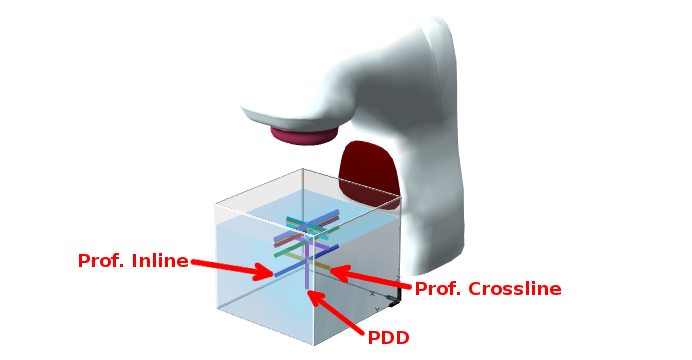
\includegraphics[height=5cm]{./img/Prof3D_ann.png}
\begin{itemize}
\scriptsize
\item \structure{\normalfont \textit{Percentage-Depth-Dose o PDD:}} si ottiene muovendo il detector (camera a ionizzazione) lungo l'asse del fascio e registrando la dose in punti con step di $\sim 1\,mm$.
\item \structure{\normalfont \textit{Profili di dose:}} si ottengono muovendo il detector in piani perpendicolari all'asse del fascio a varie profondità.
\end{itemize}
\end{frame}


\begin{frame}{Modellizzazione del LINAC}
\begin{itemize}
\scriptsize
\setbeamercolor{item}{fg=red}
\item \alert{Dosimetria del LINAC}
\end{itemize}
\vspace{.75cm}
\centering
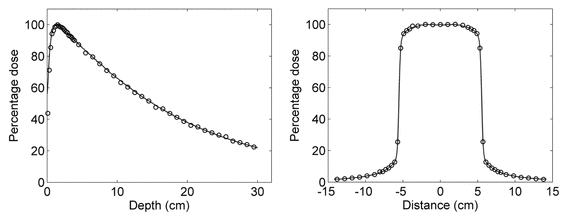
\includegraphics[height=3.5cm]{../cap2/pdd_prof.png}\\
\vspace{.75cm}
\begin{itemize}
\scriptsize
\item[a)] \structure{\normalfont \textit{Percentage-Depth-Dose o PDD:}} si ottiene muovendo il detector (camera a ionizzazione) lungo l'asse del fascio e registrando la dose in punti con step di $\sim 1\,mm$.
\item[b)] \structure{\normalfont \textit{Profili di dose:}} si ottengono muovendo il detector in piani perpendicolari all'asse del fascio a varie profondità.
\end{itemize}
\end{frame}




\begin{frame}{Modellizzazione del LINAC}
\begin{itemize}
\scriptsize
\setbeamercolor{item}{fg=red}
\item \alert{Dosimetria del LINAC}
\end{itemize}
\vspace{.75cm}
\centering
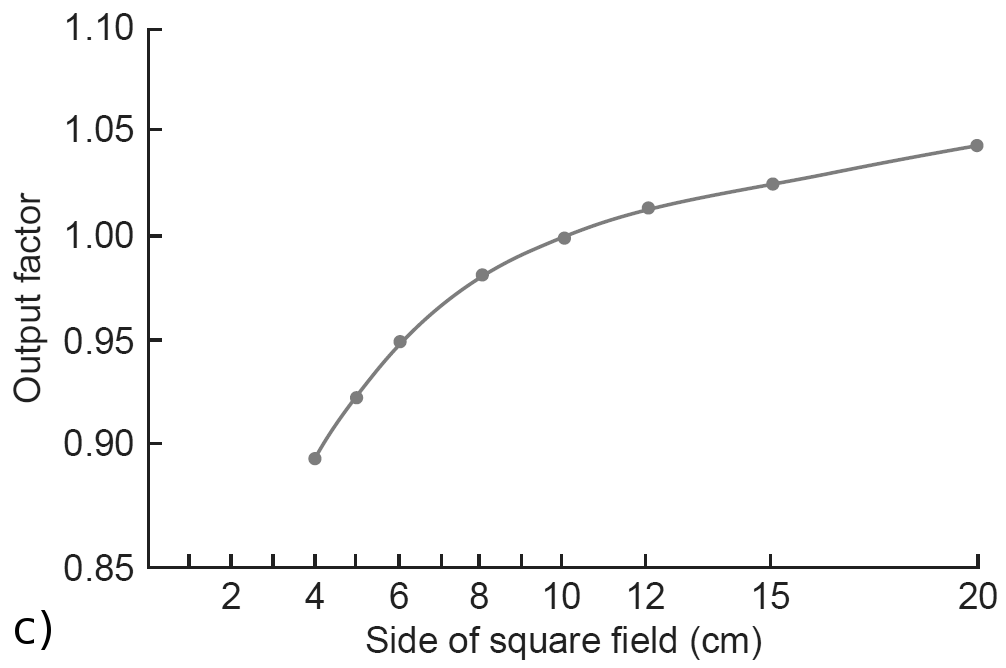
\includegraphics[height=3.5cm]{../cap2/of.png}
\scriptsize
$$\text{d)}\qquad D(Gy) = M_{raw}\,N_{d,w}\,k_{Q,Q_0}\,k_{TP}\,k_h\,k_{pol}\,k_{sat}\qquad (\textrm{IAEA TRS-398})$$
\begin{itemize}
\scriptsize
\item[c)] \structure{\normalfont \textit{Output factor:}} misure relative dell'intensità del fascio al variare delle dimensioni del campo di irradiazione.
\item[d)] \structure{\normalfont Dose assoluta (in Gy):} misura che trasforma tutte le curve di dose relativa in dose assoluta.
\end{itemize}
\end{frame}



\begin{frame}{Modellizzazione del LINAC}
\begin{itemize}
\scriptsize
\setbeamercolor{item}{fg=red}
\item \alert{Dosimetria del LINAC}
\end{itemize}
\vspace{.75cm}
\centering
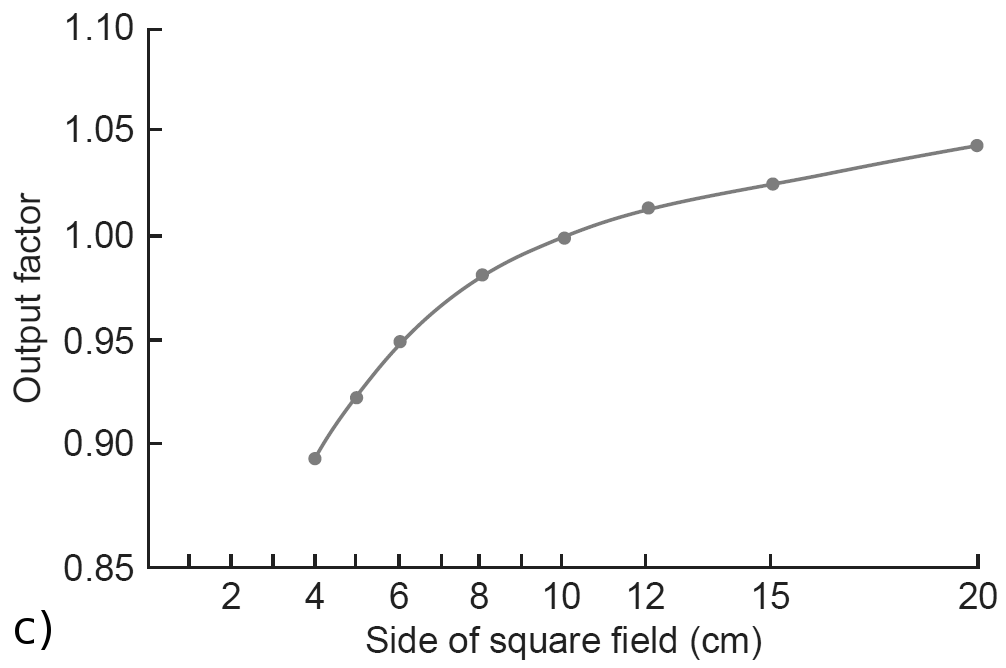
\includegraphics[height=3.5cm]{../cap2/of.png}
\scriptsize
$$\text{d)}\qquad D(Gy) = M_{raw}\,N_{d,w}\,k_{Q,Q_0}\,k_{TP}\,k_h\,k_{pol}\,k_{sat}\qquad (\textrm{IAEA TRS-398})$$
\begin{itemize}
\scriptsize
\item[c)] \structure{\normalfont \textit{Output factor:}} misure relative dell'intensità del fascio al variare delle dimensioni del campo di irradiazione.
\item[d)] \structure{\normalfont Dose assoluta (in Gy):} misura che trasforma tutte le curve di dose relativa in dose assoluta.
\end{itemize}
\end{frame}




\begin{frame}[t]{Modellizzazione del LINAC}
\begin{itemize}
\scriptsize
\setbeamercolor{item}{fg=red}
\item \alert{\textit{Tuning dei parametri} del modello del LINAC implementato nel TPS}
\end{itemize}
\vspace{.2cm}

\footnotesize
\structure{Scopo:} riprodurre le misure dosimetriche.\\\vspace{.2cm}
\alert{\textbf{Problema:}} quale accuratezza è richiesta?\\
\only<2->{
\begin{center}
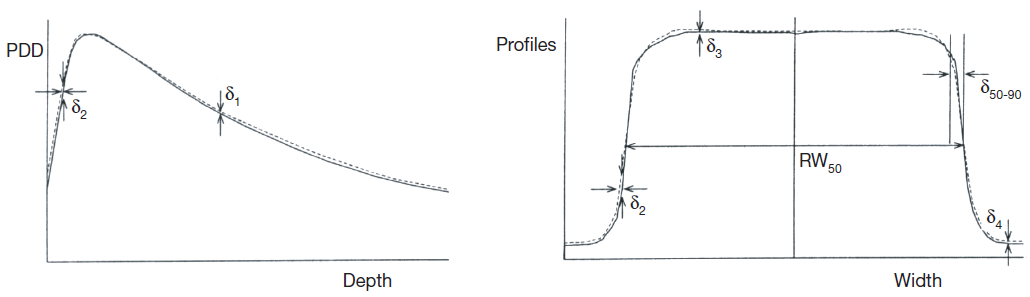
\includegraphics[width=.9\textwidth]{../cap2/Accuracy_pdd_prof.png}
\end{center}
{\color{Dgreen} Distinzione in zone:}
\begin{itemize}
\scriptsize
\item  Centro Asse, Alta dose, Basso gradiente ($\delta_1 \sim 2\% \div 4\%$).
\item  Alta dose, Alto gradiente ($\delta_2 \sim (10\%)2mm \div (15\%)3mm $).
\item  Fuori Asse, Alta dose, Basso gradiente ($\delta_3 \sim 3\% \div 4\%$).
\item  Fuori Asse, Bassa dose, Basso gradiente ($\delta_4 \sim 3\% \div 5\%$).
\end{itemize}
}
\end{frame}




\begin{frame}{Modellizzazione del LINAC}
\begin{itemize}
\scriptsize
\setbeamercolor{item}{fg=red}
\item \alert{\textit{Tuning dei parametri} del modello del LINAC implementato nel TPS}
\end{itemize}
\vspace{.5cm}
\centering
\includegraphics[width=.8\textwidth]{../cap2/ModelingSteps/ModelingSteps.eps}
\end{frame}



\begin{frame}{Modellizzazione del LINAC}
\begin{itemize}
\scriptsize
\setbeamercolor{item}{fg=red}
\item \alert{\textit{Tuning} dei parametri del modello del LINAC implementato nel TPS}
\end{itemize}
\vspace{.5cm}
\centering
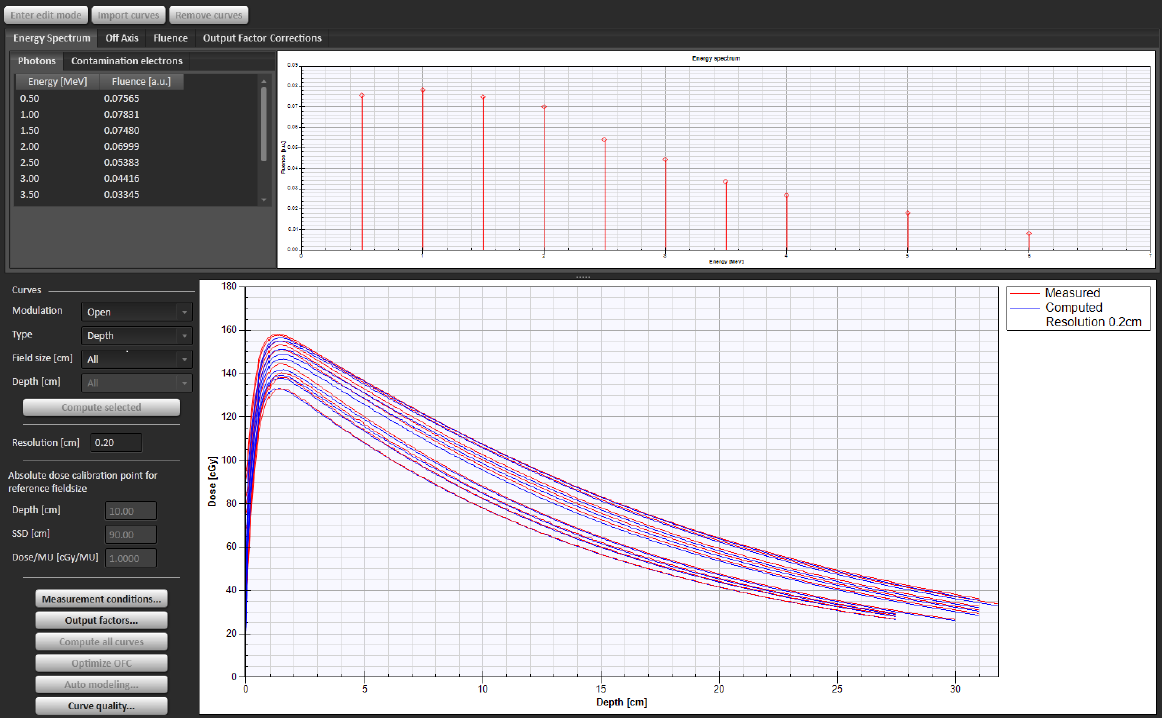
\includegraphics[width=\textwidth]{./img/RayPhysics_gui.PNG}
\end{frame}



\begin{frame}[t]{Modellizzazione del LINAC}
\footnotesize
\alert{\textbf{Problema:}} dosimetria dei piccoli campi per tecniche ad intensità modulata (IMRT).
\begin{center}
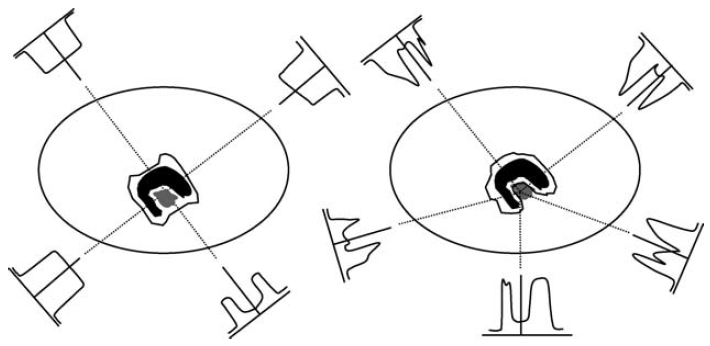
\includegraphics[width=.6\textwidth]{../cap2/3D_IMRT.png}\\\vspace{.3cm}
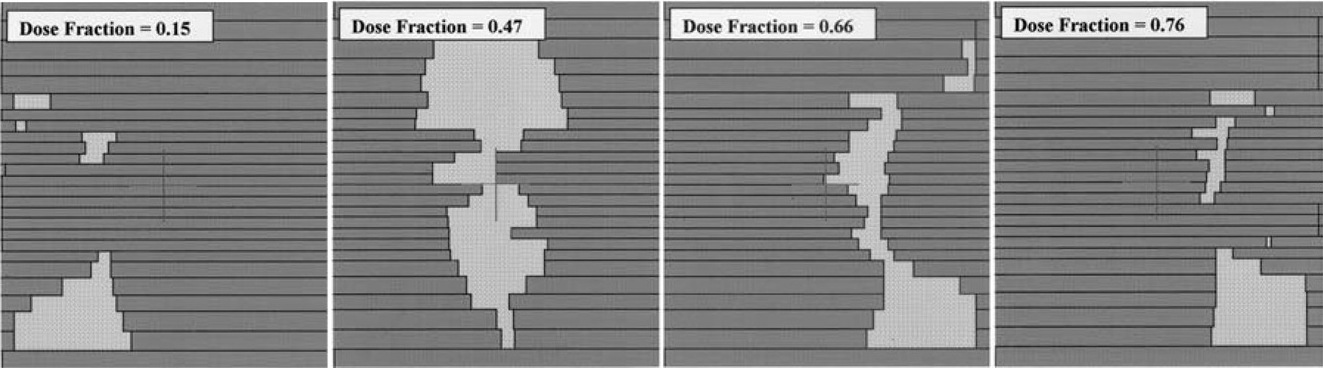
\includegraphics[width=.6\textwidth]{../cap2/IMRT_Segments_2.jpg}
\end{center}
\uncover<2->{
{\color{Dgreen} \bf Effetti:} 
\begin{itemize}
\scriptsize
\item Parziale oscuramento della sorgente $\rightarrow$ brusca caduta dell'output factor.
\item Dimensioni del campo comparabili con le dimensioni del detector $\rightarrow$ effetto di \textit{volume-averaging}.
\item Mancanza di equilibrio elettronico laterale $\rightarrow$ maggior incertezza nelle misure dosimetriche.
\end{itemize}
}
\end{frame}



\begin{frame}[t]{Modellizzazione del LINAC}
\footnotesize
\structure{Soluzione:} Misure con vari detector di nuova generazione.
metti grafico OF e poi grafico tagliato e parlare della scelta fatta fino al 2x2....

\end{frame}








\section[La radioterapia adattiva]{La radioterapia adattiva, implementazione iniziale e sviluppi futuri}
\begin{frame}{Indice}
\tableofcontents[currentsection]
\end{frame}

\begin{frame}{bla bla}
bla bla
\end{frame}

\end{document}